\chapter{Object Detection}
\section{Giới thiệu}
Object detection, còn có tên gọi là nhận diện vật thể, là một trong những lĩnh vực quan trọng của Trí tuệ nhân tạo (Artificial Intelligence) là thị giác máy (Computer Vision), đề cập đến khả năng của hệ thống máy tính và phần mềm để định vị các đối tượng trong một hình ảnh và xác định từng đối tượng. Khác với việc phân loại các vật thể ra thành từng loại riêng biệt, object detection sẽ cố gắng vẽ các bounding box xung quanh đối tượng để xác định vị trí của nó trong ảnh. \par

\begin{figure}[H]
\begin{center}
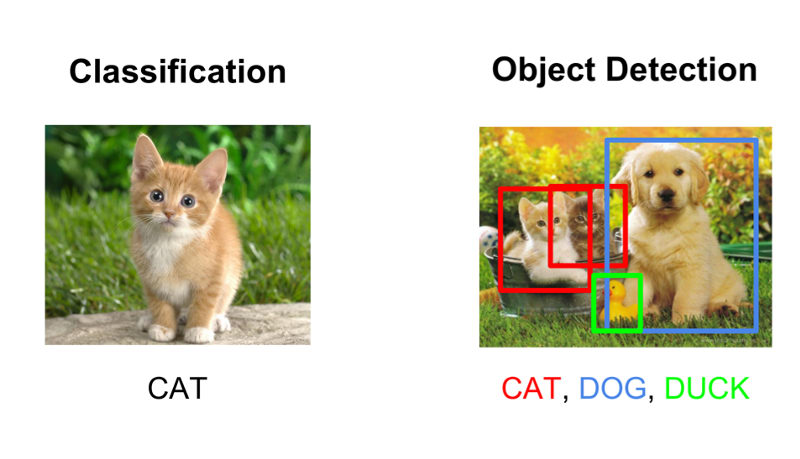
\includegraphics[scale=0.5]{chap4/image/classificationAndetection.png}
\end{center}
\caption{Phân loại và nhận diện vật thể}
\end{figure}
Object Detection đã được sử dụng rộng rãi để phát hiện khuôn mặt, phát hiện xe, đếm số người đi bộ, hệ thống bảo mật và xe không người lái. Giống như mọi công nghệ khác, một loạt các ứng dụng sáng tạo và tuyệt vời của object detection được phát triển bởi các lập trình viên và các nhà phát triển phần mềm. Tuy nhiên việc sử dụng các thuật toán cổ điển với lượng lớn dữ liệu cho bài toán object detection không còn đạt được hiệu suất đủ để làm việc trong các điều kiện khác nhau.\par
\begin{figure}[H]
\begin{center}
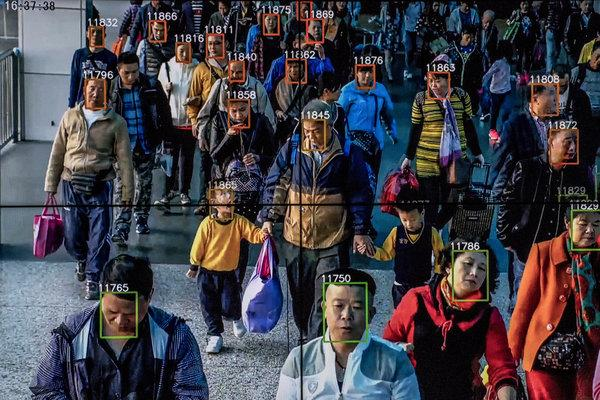
\includegraphics[scale=0.5]{chap4/image/faceDetectionChina.jpg}
\end{center}
\caption{Nhận diện khuôn mặt bên Trung Quốc}
\end{figure}
Với sự bùng nổ về dữ liệu cũng như sự đột phát và nhanh chóng về phát triển các thuật toán của học sâu vào năm 2012 đã giải quết bài toán object detection tốt hơn và chính xác cao hơn như R-CNN, Fast-RCNN, Faster-RCNN, RetinaNet, nhanh hơn nữa nhưng cũng rất chính xác như SSD và YOLO. Tôi xin trình bày sơ lược một số thuật toán điển hình.
\section{R-CNN}
R-CNN (Regions with CNN features) \cite{rcnn} là một cách tiếp cận tự nhiên nhất để giải quyết bài toán object detetion. Nó sẽ chọn ra các vùng quan tâm (regions of interest) khác nhau từ hình ảnh và sử dụng CNN để phân loại sự hiện diện của đối tượng trong khu vực đó.\par
Để giải quyết vấn đề phải chọn một số lượng lớn các vùng cần quan tâm, Ross Girshick đã đề xuất một cách giải quết đó là sử dụng thuật toán selective search \cite{van2011segmentation} để trích xuất ra chỉ 2000 vùng ở trong ảnh và tác giả gọi đó là các vùng đề xuất (region proposals). 
\begin{figure}[H]
\begin{center}
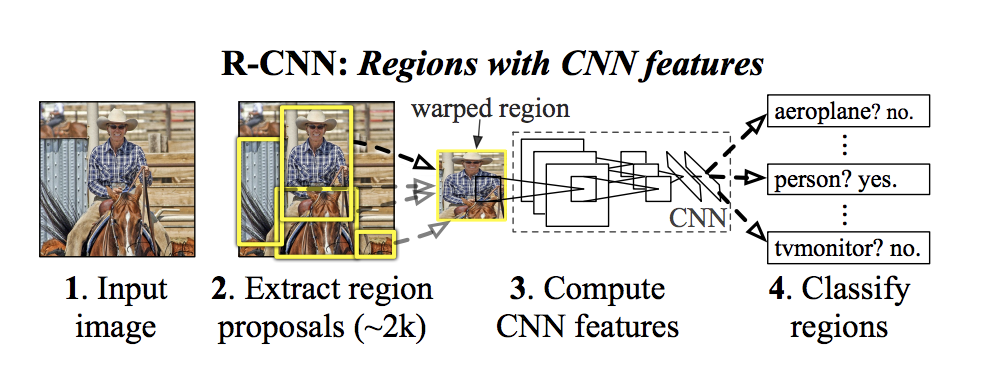
\includegraphics[scale=0.3]{chap4/image/rcnn.png}
\caption{R-CNN}
\end{center}
\end{figure}
 
2000 vùng đề xuất này sẽ được thay đổi kích thước bằng với kích thước đầu vào của các mạng đã được huấn luyện sẵn như Alex-net, VGG-16 để tính toán feed-forward các regions thu được convolutional features của mỗi region. Lúc này, CNN đóng vai trò trích xuất các đặc trưng và lớp fully-connected sử dụng các đặc trưng được trích xuất được đưa vào SVM để phân loại sự xuất hiện của đối tượng trong đề vùng được đề xuất. Ngoài việc dự đoán sự xuất hiện một đối tượng trong các đề xuất khu vực, thuật toán cũng đưa ra dự đoán bốn giá trị là tọa đô tâm, chiều cao, chiều rộng của bounding box để tăng độ chính xác của bouding box trong vùng đề xuất.\par
\begin{figure}[H]
\begin{center}
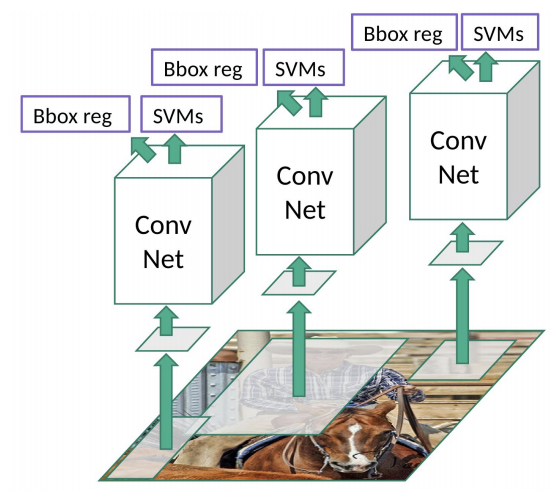
\includegraphics[scale=0.5]{chap4/image/rcnn2.png}
\caption{R-CNN}
\end{center}
\end{figure}
\textbf{Vấn đề của R-CNN}
\begin{itemize}
\item[-]Nó sẽ tiêu tốn một lượng lớn thời gian để huấn luyện do bạn phải thực phân loại 2000  region proposals mỗi ảnh.
\item[]Nó không thực hiện được trên thời gian thực do tiêu tốn 47 giây cho mỗi lần đánh giá một ảnh.
\item[]Thuật toán selective search \cite{van2011segmentation} là một thuật toán cố định, ở trạng thái này việc học sẽ không xảy ra. Do đó nó có thể tạo cho chúng ta những region proposals không tốt.
\end{itemize}
\section{Fast R-CNN}
%\begin{figure}[H]
%\begin{center}
%\label{fig:convFeatureMap}
%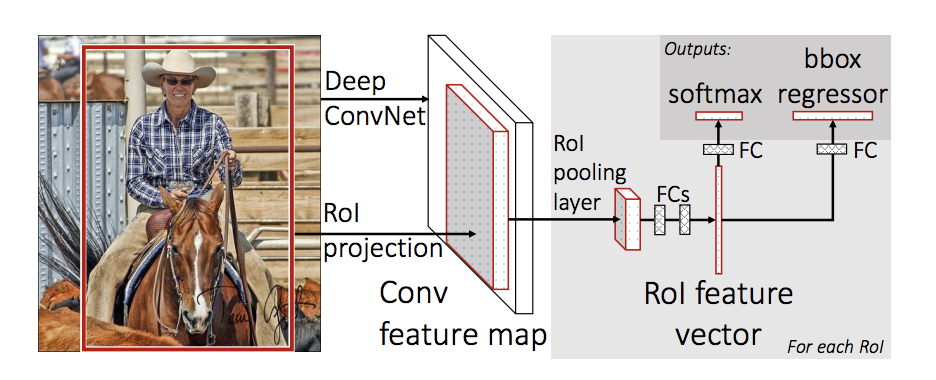
\includegraphics[scale= 0.5]{chap4/image/fastrcnn.png}
%\caption{Fast R-CNN}
%\end{center}
%\end{figure}
Fast R-CNN giải quyết một số nhược điểm của R-CNN để xây dựng thuật toán object detection nhanh hơn và do đó nó có tên gọi là như vậy. Cách tiếp cận tương tự như thuật toán R-CNN, thay vì sử dụng các region proposals được tạo ra ngay ở ảnh gốc, ta lấy ảnh gốc làm đầu vào cho CNN và tạo convolutional feature map.
\begin{figure}[H]
\begin{center}
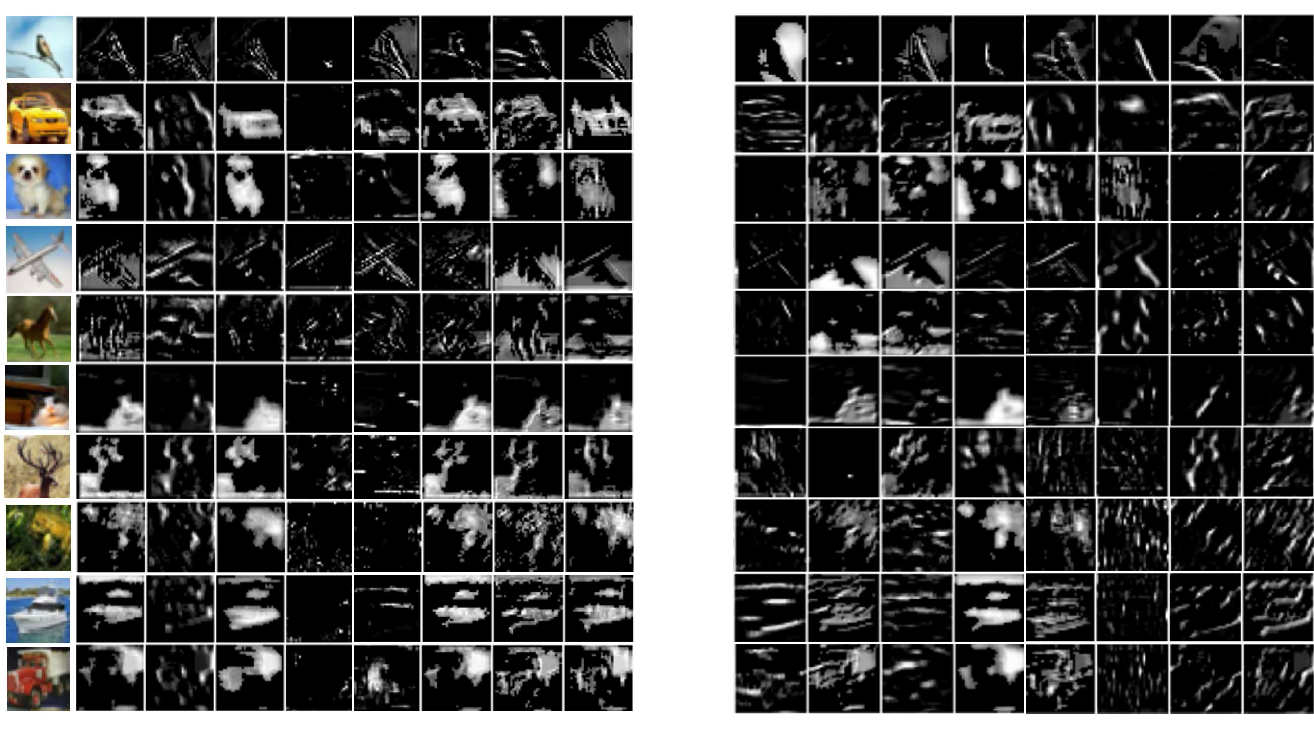
\includegraphics[scale=0.4]{chap4/image/featureMap.png}
\end{center}
\caption{Convolutional feature map}
\label{fig:convFeatureMap11}
\end{figure}
Từ các convolutional feature map này ta sử dụng thuật toán selective search để tạo ra các region of proposals và sử dụng tầng RoI pooling để đưa các convolutional feature map thành đầu vào cho tầng fully-connected và đưa ra dự đoán bounding box.
\begin{figure}[H]
\begin{center}
\label{fig:convFeatureMap}
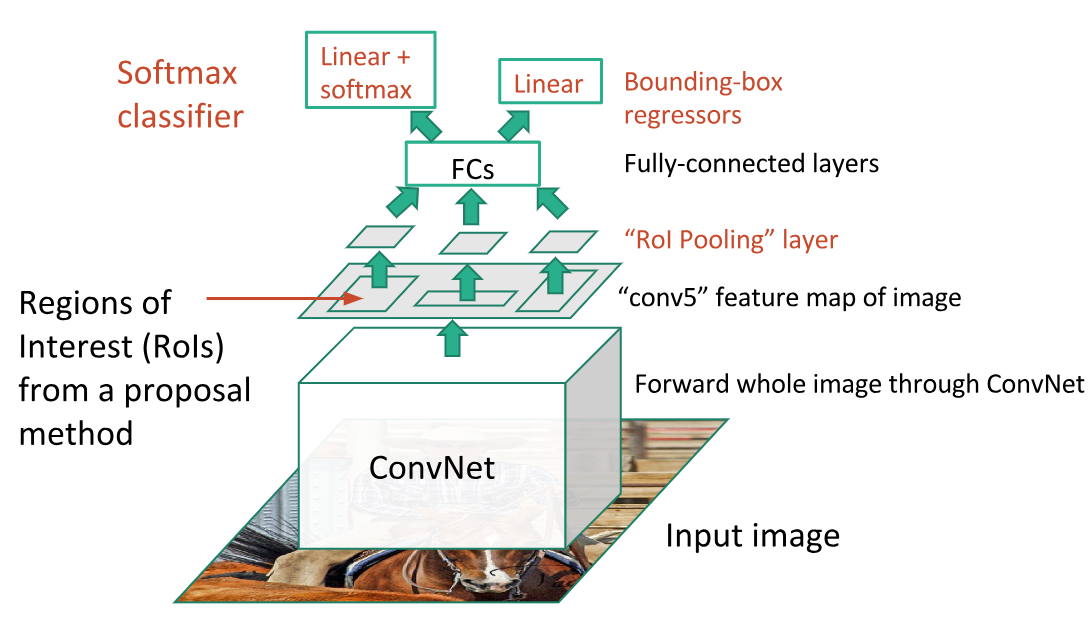
\includegraphics[scale= 0.8]{chap4/image/fastrcnn2.png}
\caption{Fast R-CNN}
\end{center}
\end{figure}
Lý do Fast R-CNN nhanh hơn R-CNN là do chúng ta không phải thực hiện 2000 lần chạy CNN cho mỗi ảnh mà thay vào đó ta sẽ chỉ sử dụng một lần chạy CNN với đầu vào là ảnh gốc và khi đã có được feauture map thì ta mới tạo ra các region proposals.
\begin{figure}[H]
\begin{center}
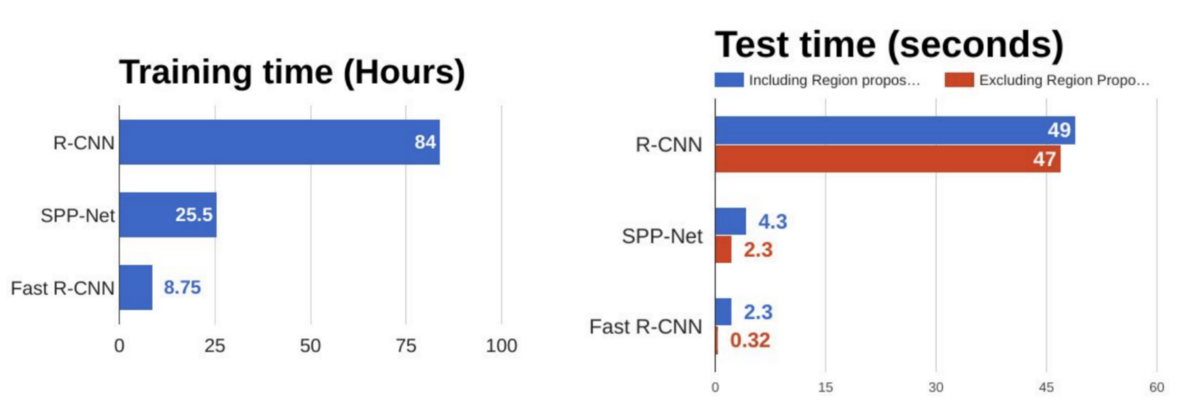
\includegraphics[scale=0.3]{chap4/image/hieusuat.png}
\caption{So sánh tốc độ huấn luyện và đánh giá của các thuật toán}
\end{center}
\end{figure}
\section{Faster R-CNN}
Faster R-CNN được phát triển từ Fast R-CNN giúp cải thiện tốc độ và độ chính xác. Sự cải tiến của thuật toán đó là thay vì sử dụng selective search để tạo ra các regions proposal thì Faster R-CNN sử dụng mạng RPN (Region Proposal Network).
\begin{figure}[H]
\begin{center}
\label{fig:convFeatureMap}
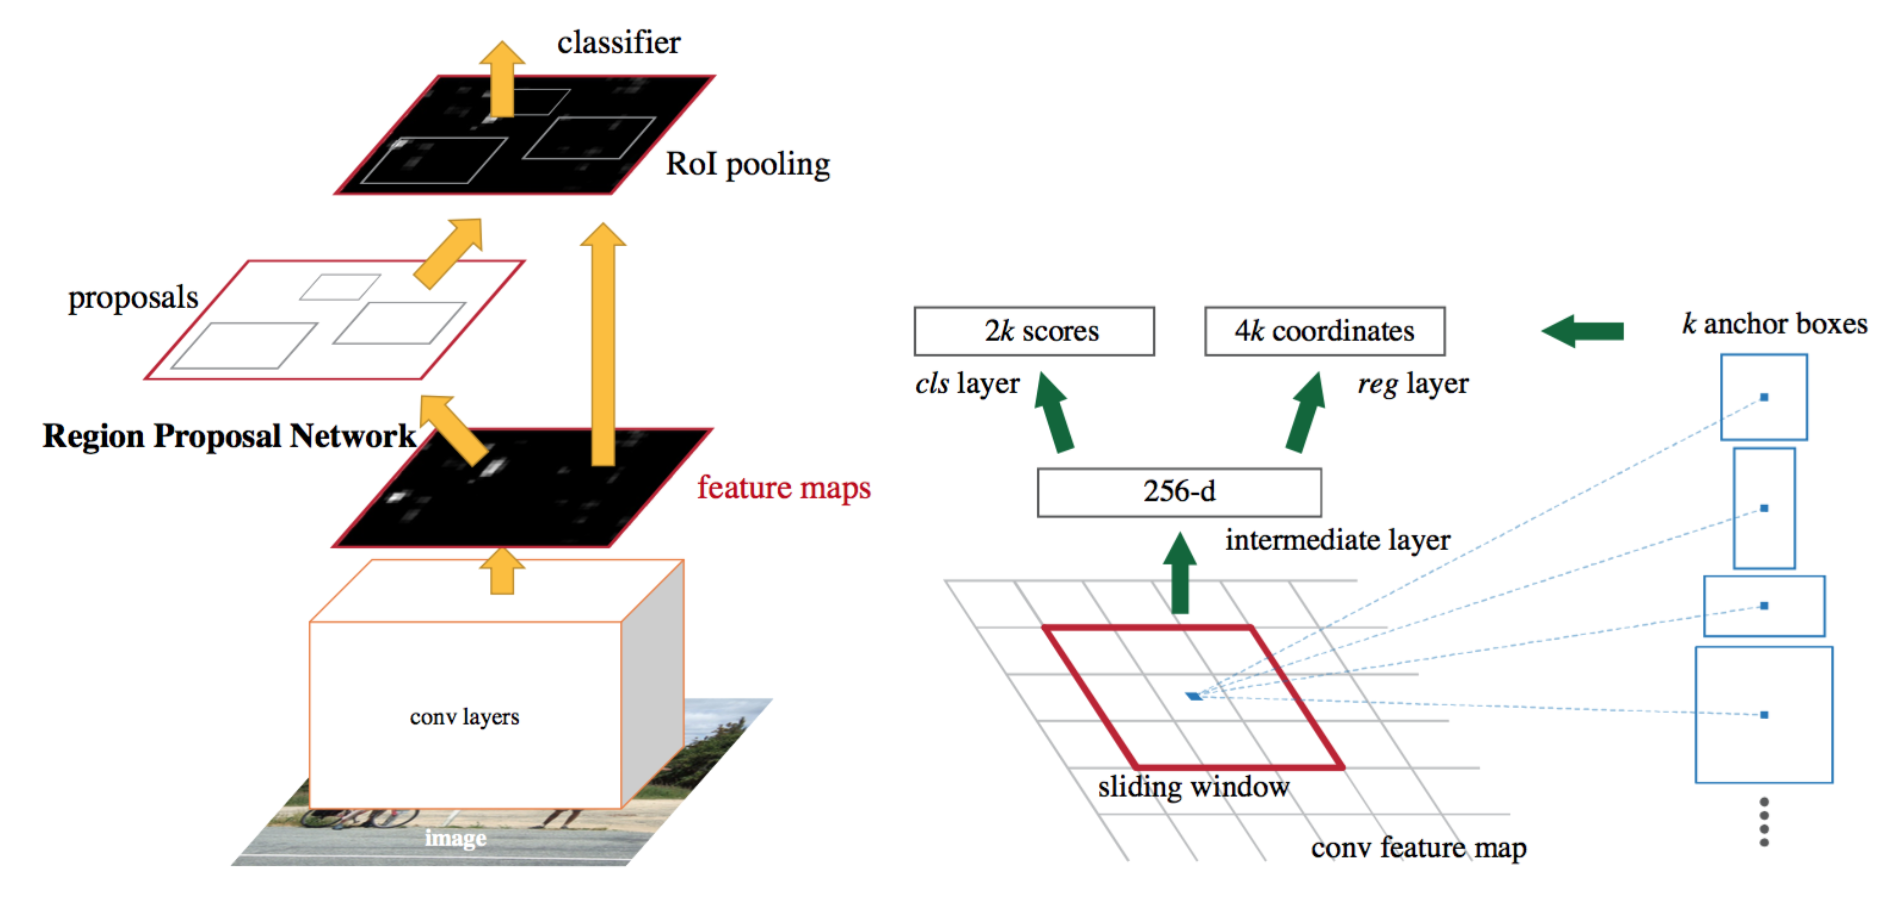
\includegraphics[scale= 0.5]{chap4/image/fasterrcnn.png}
\caption{Faster R-CNN}
\end{center}
\end{figure}
%\labeltext{RPN}{\label{text:rpn}}
RPN sử dụng feauture map để làm đầu vào và dùng bộ lọc trượt trên đó. Mỗi bước trượt sẽ tạo ra thêm $k$ region proposals theo tỉ lệ định trước và các region proposals đó được gọi là các anchor boxes. Tại thuật toán Faster R-CNN, số anchor boxes được tạo ra ở mỗi bước trượt là 9 anchor boxes. Khi đã thu được đầu ra của các anchor boxes, ta tính độ chính xác của anchor boxes dựa vào tỉ lệ diện tích giữa anchor box đè ground truth so với tổng diện tích của anchorbox và ground truth. Cách tính này được gọi là intersection over union (IoU)

\begin{figure}[H]
\begin{center}
\label{fig:iou}
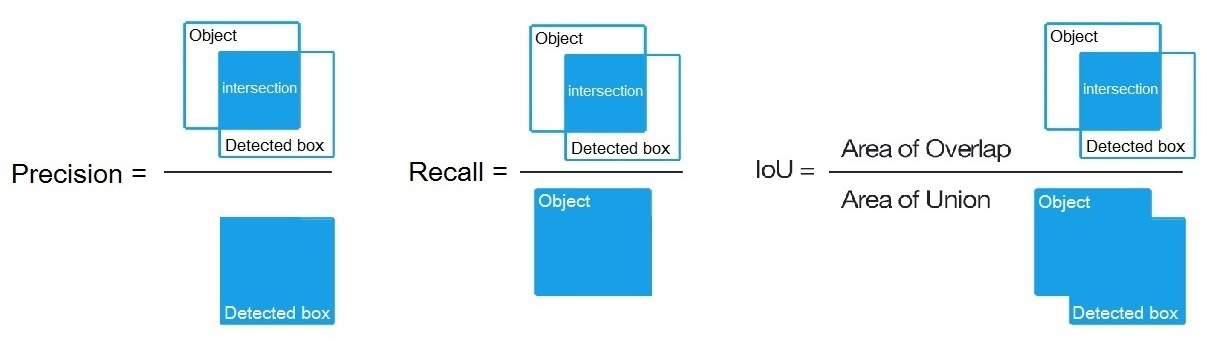
\includegraphics[scale=0.4]{chap4/image/iou.jpg}
\caption{Intersection over union (IoU)}
\end{center}
\end{figure}
	
\begin{figure}[H]
\begin{center}
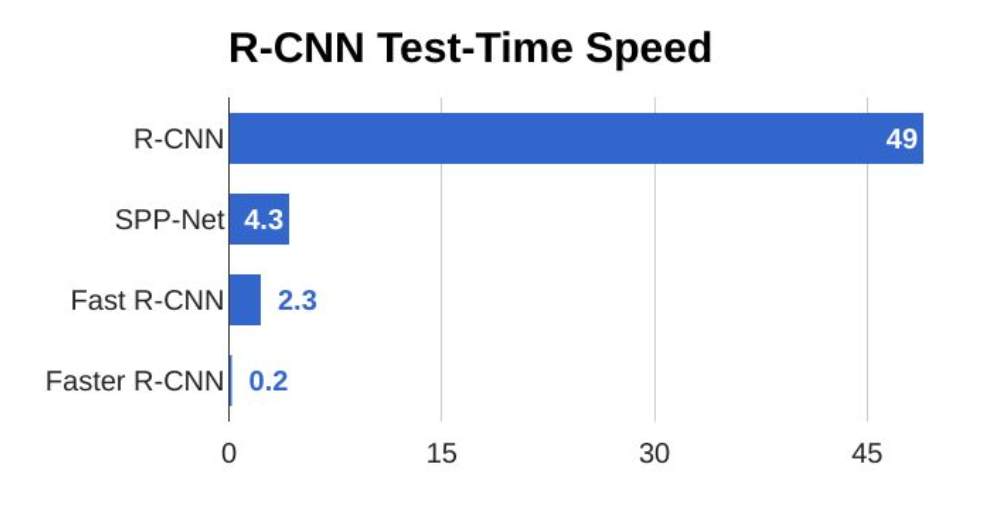
\includegraphics[scale=0.6]{chap4/image/hieusuat2.png}
\caption{So sánh thời gian thực nghiệm của các thuật toán}
\end{center}
\end{figure}
\section{YOLO}
Không giống như những thuật toán trước, yolo chỉ sử dụng duy nhất một mạng CNN để nhận diện và dự đoán vật thể vì thế nó có tên gọi là you only look once. Và yolo có thể nhận diện và phân loại vật thể trên thời gian thực với độ chính xác cao.\par
Yolo chia ảnh thành lưới các ô vuông có kích thước là $n\times n $. Tại mỗi ô vuông ta tạo ra thêm $k$ anchor boxes giống như RPN.
%(\ref{text:rpn}).
\begin{figure}[H]
\begin{center}
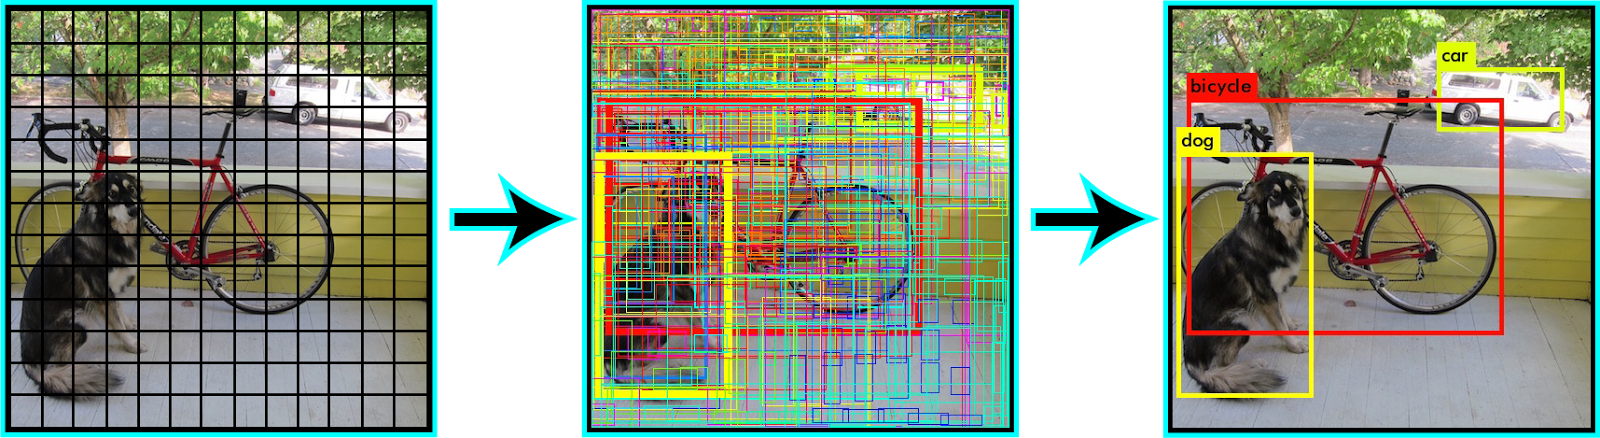
\includegraphics[scale=0.3]{chap4/image/yolo1.png}
\end{center}
\caption{Yolo}
\end{figure}

Nếu tâm của object nằm trong một ô vuông thì ô vuông đó sẽ chịu trách nhiệm phát hiện ra object này. Giả sử chúng ta cần phân ra 3 loại object: $c1$, $c_2$, $c_3$; khi đó mỗi anchor boxes sẽ được đưa vào mạng CNN và trả ra đầu ra có dạng là
\begin{align*}
y = 
\begin{bmatrix}
p_c\\
b_x\\
b_y\\
b_w\\
b_h\\
c_1\\
c_2\\
c_3\\
\end{bmatrix}
\end{align*}
trong đó $p_c$ là xắc suất rơi vào class $c$; $b_x$, $b_y$ là tọa độ dự đoán tâm object; $b_h$, $b_w$ là kích thước tương ứng của object so với chiều cao và chiều rộng của ô vuông.\par
Nếu ta có nhiều anchor boxes cho mỗi ô thì ta sẽ thu được đầu ra là bằng với số lượng phần tử trên nhân với số lượng anchor boxes.
\begin{figure}[H]
\begin{center}
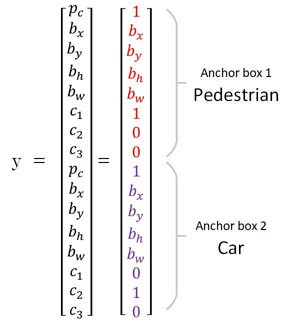
\includegraphics[scale=0.6]{chap4/image/labelyolo.jpg}
\caption{Ví dụ nhãn với anchor box = 2}
\end{center}
\end{figure}
Khi đã có đầu ra của từng anchor boxes, ta sử dụng IoU để chọn ra anchor box mỗi lớp có xắc suất cao nhất, các anchor boxes cung lớp khác sẽ bị loại bỏ.